% !TEX program = xelatex
%% 基于声音的鸟类识别系统 — 项目报告
%% 使用 jcip-latex-template-master 模板
%% 编译命令：xelatex main.tex

\documentclass[10pt,twoside,twocolumn]{article}

% ── 中文与字体 ──────────────────────────────────────────────
\usepackage{ctex}
\usepackage{fontspec}

% ── 页面与基础宏包 ──────────────────────────────────────────
\usepackage[
  a4paper,
  top=28mm, bottom=25mm,
  left=19mm, right=19mm,
  columnsep=6mm,
  headsep=6mm,
  headheight=24pt,
  footskip=10mm
]{geometry}

\usepackage{amsmath,amssymb,bm}
\usepackage{graphicx}
\usepackage{booktabs}
\usepackage{caption}
\usepackage{fancyhdr}
\usepackage{titlesec}
\usepackage{indentfirst}
\usepackage{cite}
\usepackage{url}
\usepackage{xcolor}
\usepackage{listings}   % 代码高亮

\graphicspath{{../results/}}

\captionsetup{font=small,labelfont=bf,labelsep=space}
\captionsetup[figure]{position=below,name=图}
\captionsetup[table]{position=above,name=表}
\setlength{\parindent}{2em}

% ── 代码样式 ──────────────────────────────────────────────
\lstset{
  basicstyle=\zihao{-6}\ttfamily,
  breaklines=true,
  frame=single,
  xleftmargin=1em,
  xrightmargin=0.5em,
  numbers=left,
  numberstyle=\tiny,
  keywordstyle=\color{blue!80}\bfseries,
  commentstyle=\color{gray},
  stringstyle=\color{red!70},
  language=Python,
  showstringspaces=false
}

% ── 期刊信息 ────────────────────────────────────────────────
\newcommand{\jcipvol}{**}
\newcommand{\jcipno}{*}
\newcommand{\jcipyear}{2026}
\newcommand{\jcipmonth}{6}
\newcommand{\articleno}{语音识别技术大作业}

\newcommand{\runningtitletext}{基于声音的鸟类识别系统}
\newcommand{\runningtitle}[1]{\gdef\runningtitletext{#1}}

% ── 页眉页脚 ────────────────────────────────────────────────
\pagestyle{fancy}
\fancyhf{}
\fancyhead[LE]{\zihao{-5}\thepage\quad 语音识别技术}
\fancyhead[CE]{\zihao{-5}\runningtitletext}
\fancyhead[RO]{\zihao{-5}2026年\ 大作业}
\fancyhead[CO]{\zihao{-5}\runningtitletext}
\fancyfoot[LE,RO]{\zihao{-5}\thepage}
\renewcommand{\headrulewidth}{0.4pt}

\fancypagestyle{jcipfirst}{%
  \fancyhf{}
  \fancyhead[C]{\zihao{-5}\textbf{语音识别技术课程大作业报告}\\[-1pt]
    \small SPEECH RECOGNITION TECHNOLOGY --- FINAL PROJECT}
  \fancyfoot[C]{\zihao{6}南京师范大学\ \jcipyear 年}
  \renewcommand{\headrulewidth}{0.4pt}
}

% ── 标题样式 ────────────────────────────────────────────────
\titleformat{\section}{\zihao{-4}\heiti}{\thesection}{1em}{}
\titleformat{\subsection}{\zihao{5}\heiti}{\thesubsection}{1em}{}
\titleformat{\subsubsection}{\zihao{5}\songti}{\thesubsubsection}{1em}{}
\setcounter{secnumdepth}{3}

% ── 摘要环境 ────────────────────────────────────────────────
\renewenvironment{abstract}{%
  \noindent{\zihao{-5}\heiti 摘要：}\zihao{-5}\kaishu\ignorespaces
}{\par\medskip}

\newenvironment{enabstract}{%
  \noindent{\zihao{-5}\textbf{Abstract: }}\zihao{-5}\ignorespaces
}{\par\medskip}

\newcommand{\keywords}[1]{%
  \noindent{\zihao{-5}\heiti 关键词：}{\zihao{-5}\kaishu #1}\par\smallskip}
\newcommand{\enkeywords}[1]{%
  \noindent{\zihao{-5}\textbf{Key words: }}{\zihao{-5} #1}\par\medskip}
\newcommand{\clccode}[2]{%
  \noindent{\zihao{-5}\heiti 中图分类号：}{\zihao{-5}#1}%
  \hfill{\zihao{-5}\heiti 文献标识码：}{\zihao{-5}#2}\par\bigskip}

% ── 作者简介 ────────────────────────────────────────────────
\newlength{\photow}\newlength{\photoh}
\setlength{\photow}{1.8cm}\setlength{\photoh}{2.4cm}
\newcommand{\authorentry}[2]{%
  \par\noindent
  \begin{minipage}[t]{\photow}
    \fbox{\rule{0pt}{\photoh}\rule{\dimexpr\photow-2\fboxsep-2\fboxrule\relax}{0pt}}
  \end{minipage}%
  \hspace{4pt}%
  \begin{minipage}[t]{\dimexpr\linewidth-\photow-4pt\relax}
    \zihao{6}#2
  \end{minipage}\par\smallskip}

% ════════════════════════════════════════════════════════════
\begin{document}
\thispagestyle{jcipfirst}
\runningtitle{基于声音的鸟类识别系统}

% ── 题头区（单栏） ─────────────────────────────────────────
\twocolumn[{%
  \begin{center}
    {\zihao{3}\heiti 基于声音的鸟类识别系统}\par\medskip
    {\zihao{4}\songti 徐圣童$^{1}$}\par\smallskip
    {\zihao{-5}\songti
      （1. 南京师范大学计算机与电子信息/人工智能学院，江苏\ 南京\ 210023）
    }\par\medskip
  \end{center}

  \begin{abstract}
该文基于BirdCLEF 2026数据集，构建了一套完整的基于声音的鸟类识别系统。
首先对音频进行预处理（重采样至22\,050\,Hz、截取/填充至5\,s），
提取包括梅尔频率倒谱系数（Mel-frequency Cepstral Coefficient，MFCC）
及其一阶、二阶差分、基频（F0）、均方根能量（Root Mean Square，RMS）、
频谱质心/带宽/滚降/平坦度和过零率（Zero Crossing Rate，ZCR）共278维声学特征。
在此基础上分别构建了K近邻（K-Nearest Neighbor，KNN）、
支持向量机（Support Vector Machine，SVM）、
随机森林（Random Forest，RF）等传统机器学习模型，
以及基于对数梅尔频谱图的卷积神经网络（Convolutional Neural Network，CNN）
和基于MFCC序列的双向长短时记忆网络（Bidirectional Long Short-Term Memory，BiLSTM）
深度学习模型，共5种模型。
实验结果表明，CNN模型取得最优性能，测试集准确率为48.75\%，
宏平均F1分数（Macro F1）为0.463，优于其他所有模型。
深度学习方法整体优于传统机器学习方法，验证了端到端特征学习的有效性。
最后，该文使用Gradio构建了Web交互界面，支持实时音频上传与多模型识别结果展示。
  \end{abstract}

  \keywords{鸟类识别；声音识别；梅尔频率倒谱系数；卷积神经网络；双向长短时记忆网络}
  \clccode{TP391}{A}

  \begin{center}
    {\zihao{4}\textit{Bird Species Recognition System Based on Sound}}\par\medskip
    {\zihao{5} Choi Seng Tong$^{1}$}\par\smallskip
    {\zihao{-5}
      (1. School of Computer and Electronic Information/School of Artificial Intelligence, Nanjing Normal University, Nanjing 210023, China)
    }\par\medskip
  \end{center}

  \begin{enabstract}
This paper presents a bird sound recognition system based on the BirdCLEF 2026 dataset.
Audio clips are preprocessed by resampling to 22\,050\,Hz and padding/trimming to 5\,s.
A 278-dimensional acoustic feature vector is extracted, including MFCCs with
first- and second-order deltas, fundamental frequency (F0), RMS energy,
spectral centroid/bandwidth/rolloff/flatness, and zero-crossing rate (ZCR).
Three traditional machine learning models (KNN, SVM, Random Forest) and
two deep learning models---CNN on log-Mel spectrograms and BiLSTM on MFCC sequences---are
constructed and compared.
Experimental results show that CNN achieves the best performance with
48.75\% test accuracy and a Macro F1 score of 0.463.
Deep learning methods outperform traditional ML methods overall,
validating the effectiveness of end-to-end feature learning.
A Gradio-based web interface is also developed for real-time bird sound recognition.
  \end{enabstract}
  \enkeywords{bird recognition; sound recognition; MFCC; CNN; BiLSTM}
  \bigskip
}]

\zihao{5}\songti
\setcounter{section}{-1}

% ════════════════════════════════════════════════════════════
\section{引言}

鸟类是生态系统健康的重要指示物种，其多样性监测对生物保护具有重要意义。
传统人工野外调查效率低、成本高，难以大规模部署。
近年来，被动声学监测技术的兴起使得自动化鸟鸣识别成为可能\cite{stowell2019}。
基于机器学习的鸟鸣识别系统已在生物多样性调查中展现出广阔的应用前景。

BirdCLEF 2026是Kaggle举办的国际鸟类声音识别竞赛，
提供了来自南美洲热带地区的大规模野外鸟鸣录音数据集\cite{birdclef2026}。
该文基于此数据集，综合运用传统机器学习与深度学习方法构建多模型对比系统，
并提供Web交互界面，旨在探索不同特征表示与模型结构对鸟鸣识别性能的影响。

% ════════════════════════════════════════════════════════════
\section{数据集与预处理}

\subsection{数据集}

BirdCLEF 2026数据集收录了鸟类（Aves）、两栖类、爬行类等多种生物的声音录音，
音频格式为.ogg，来源包括iNaturalist和Xeno-canto平台。
该文从中筛选鸟类样本，选取样本数量最多的20个物种进行实验，
共涵盖Osprey（鱼鹰）、Tropical Screech Owl（热带鸣角鸮）等20种鸟类。
每类深度学习最多取100条、传统机器学习最多取50条，
共约1\,600条训练样本（见表~\ref{tab:dataset}）。

\begin{table}[h]
\caption{数据集配置}
\label{tab:dataset}
\centering\zihao{-5}
\begin{tabular}{ll}
\toprule
属性 & 说明 \\
\midrule
音频格式 & .ogg（重采样至22\,050\,Hz，单声道）\\
识别类别数 & 20种鸟类（Aves） \\
深度学习样本 & 每类$\leq$100条，共$\approx$1\,600条 \\
传统ML样本 & 每类$\leq$50条，共$\approx$800条 \\
单条音频时长 & 5\,s（零填充/截断） \\
数据划分 & 训练/验证/测试 = 8:1:1（分层） \\
\bottomrule
\end{tabular}
\end{table}

\subsection{预处理}

（1）\textbf{重采样}：使用librosa将所有音频统一重采样至22\,050\,Hz；

（2）\textbf{单声道}：立体声混合为单声道；

（3）\textbf{时长标准化}：截取或零填充至固定5\,s（110\,250采样点）；

（4）\textbf{数据划分}：按8:1:1比例进行分层随机划分，
保证各子集中各类别比例一致。

% ════════════════════════════════════════════════════════════
\section{特征提取}

\subsection{传统机器学习特征向量（278维）}

对每条5\,s音频计算以下声学特征在时间轴上的均值与标准差，
拼接成278维固定长度特征向量（见表~\ref{tab:features}）。

\begin{table}[h]
\caption{传统机器学习特征构成（278维）}
\label{tab:features}
\centering\zihao{-5}
\resizebox{\columnwidth}{!}{%
\begin{tabular}{llr}
\toprule
特征类别 & 描述 & 维度 \\
\midrule
MFCC+$\Delta$+$\Delta^2$ & 40阶及一、二阶差分（均值+标准差） & 240 \\
Chroma & 12维色度特征 & 24 \\
频谱形状 & 质心、带宽、滚降点、平坦度 & 8 \\
ZCR & 过零率，反映鸣叫速率 & 2 \\
RMS & 均方根能量，反映音量 & 2 \\
F0 (YIN) & 基频，反映音高，32--2048\,Hz & 2 \\
\midrule
合计 & & 278 \\
\bottomrule
\end{tabular}%
}
\end{table}

MFCC是从梅尔滤波器组输出的对数能量经离散余弦变换得到的倒谱系数，
能够有效压缩频谱的时频包络信息\cite{mfcc1980}。
音高（pitch）使用YIN算法\cite{yin2002}从基频轨迹估计，
仅对有声帧（$f_0>0$）统计均值与标准差，静音帧置零。

核心特征提取代码如下：

\begin{lstlisting}[caption={特征提取核心代码（utils.py节选）}]
def extract_features(y, sr=22050):
    mfcc = librosa.feature.mfcc(
        y=y, sr=sr, n_mfcc=40,
        n_fft=2048, hop_length=512)
    delta1 = librosa.feature.delta(mfcc)
    delta2 = librosa.feature.delta(mfcc, order=2)
    feats = []
    for mat in (mfcc, delta1, delta2):
        feats.extend(mat.mean(axis=1))
        feats.extend(mat.std(axis=1))
    # 音高 F0 (YIN)
    f0 = librosa.yin(y, fmin=32, fmax=2048,
                     sr=sr, hop_length=512)
    f0v = f0[f0 > 0]
    feats += [float(f0v.mean()) if len(f0v) else 0.,
              float(f0v.std())  if len(f0v) else 0.]
    return np.array(feats, dtype=np.float32)
\end{lstlisting}

\subsection{CNN输入：对数梅尔频谱图}

参数设置$n\_mels=128$、$n\_fft=2048$、$hop\_length=512$，
计算对数梅尔频谱图并固定为212帧，归一化至$[0,1]$，
形状为$(1, 128, 212)$。

\subsection{BiLSTM输入：MFCC时序矩阵}

提取40阶MFCC时序序列，对每个倒谱系数独立进行z-score标准化，
固定为212帧，形状为$(212, 40)$，保留鸣声随时间变化的动态信息。

图~\ref{fig:audio_vis}展示了典型鸟鸣音频的多种特征可视化结果。

\begin{figure}[h]
\centering
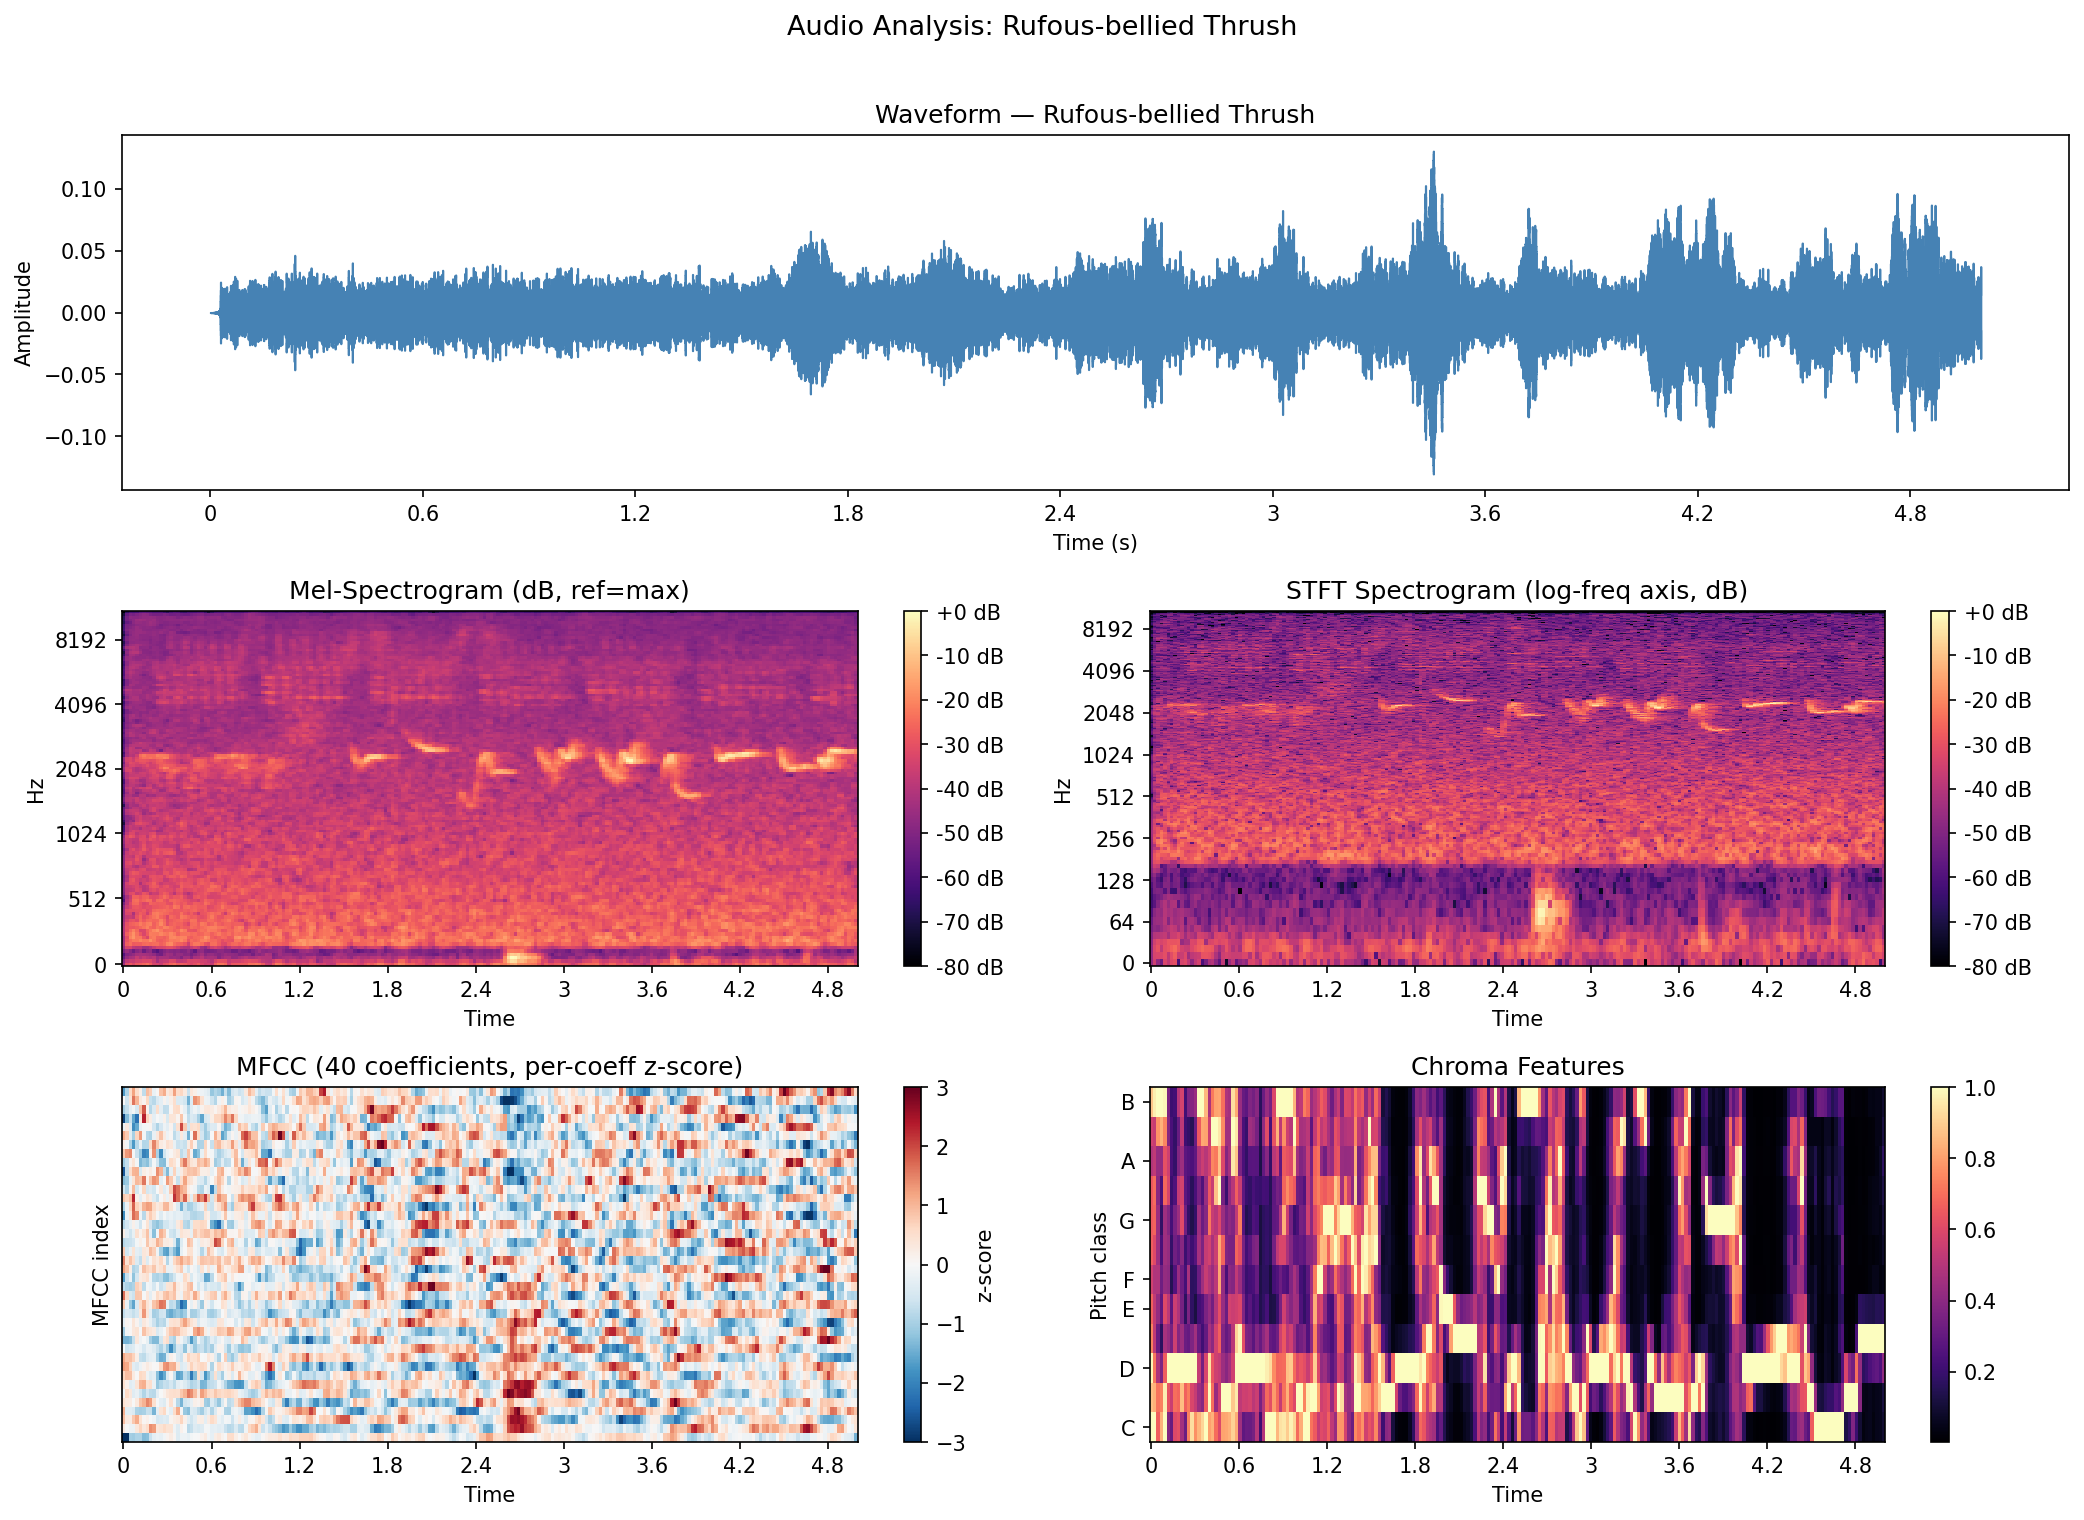
\includegraphics[width=\linewidth]{03_audio_analysis.png}
\caption{鸟鸣音频波形、梅尔频谱、MFCC与色度图}
\label{fig:audio_vis}
\end{figure}

% ════════════════════════════════════════════════════════════
\section{模型构建}

\subsection{传统机器学习模型}

三种传统模型均以278维特征向量为输入，
训练前经StandardScaler标准化，
采用5折分层交叉验证（StratifiedKFold）
结合GridSearchCV进行超参数搜索。

\textbf{KNN}：通过欧氏距离寻找$K$个最近邻居进行多数投票，
网格搜索$K\in\{3,5,7,9\}$及距离权重策略\cite{cover1967}。

\textbf{SVM}：使用RBF核将特征映射至高维空间，
寻找最大间隔决策超平面，
网格搜索$C\in\{0.1,1,10\}$和$\gamma\in\{\text{scale, auto}\}$\cite{cortes1995}。

\textbf{随机森林（RF）}：集成多棵决策树，
每棵树用Bootstrap样本和随机子特征训练，
最终多数投票，有效缓解过拟合\cite{breiman2001}。

\subsection{卷积神经网络（CNN）}

以对数梅尔频谱图作为二维图像输入。
网络由4个卷积块构成，结构为
Conv2d-BN-ReLU$\times$2 + MaxPool + Dropout，
通道数依次为32→64→128→256。
之后接AdaptiveAvgPool2d$(4\times4)$
和全连接分类头（4096→512→256→20）。
训练采用AdamW优化器（$lr=10^{-3}$，$\text{weight\_decay}=10^{-4}$）、
CosineAnnealingLR学习率调度和WeightedRandomSampler处理类别不平衡，
以验证集准确率为指标进行早停（patience=7）\cite{he2016}。

\begin{lstlisting}[caption={CNN模型结构（04\_cnn\_model.py节选）}]
class BirdCNN(nn.Module):
    def __init__(self, n_classes):
        super().__init__()
        self.features = nn.Sequential(
            nn.Conv2d(1,32,3,padding=1),
            nn.BatchNorm2d(32), nn.ReLU(),
            nn.Conv2d(32,32,3,padding=1),
            nn.BatchNorm2d(32), nn.ReLU(),
            nn.MaxPool2d(2,2), nn.Dropout2d(0.1),
            # ... (共4个卷积块)
            nn.AdaptiveAvgPool2d((4,4)),
        )
        self.classifier = nn.Sequential(
            nn.Flatten(),
            nn.Linear(256*4*4,512), nn.ReLU(),
            nn.Dropout(0.5),
            nn.Linear(512,256), nn.ReLU(),
            nn.Dropout(0.3),
            nn.Linear(256, n_classes),
        )
\end{lstlisting}

\subsection{双向长短时记忆网络（BiLSTM）+ 注意力机制}

将MFCC时序矩阵作为序列输入，
通过双向长短时记忆网络（Bidirectional LSTM）\cite{hochreiter1997}
同时建模正向与反向时序依赖。
引入注意力机制（Attention）对各时刻隐状态加权聚合，
突出关键鸣叫片段（hidden\_size=128，2层，dropout=0.3），
全连接头为256→128→20。

注意力聚合计算如式~(\ref{eq:attention})：
\begin{equation}
  \mathbf{c} = \sum_{t=1}^{T} \alpha_t \mathbf{h}_t, \quad
  \alpha_t = \frac{\exp(\mathbf{w}^\top \mathbf{h}_t)}
                  {\sum_{j=1}^{T}\exp(\mathbf{w}^\top \mathbf{h}_j)}
  \label{eq:attention}
\end{equation}
其中$\mathbf{h}_t$为第$t$时刻双向LSTM的隐状态，$\mathbf{w}$为可学习参数向量。

% ════════════════════════════════════════════════════════════
\section{实验结果与分析}

\subsection{传统机器学习结果}

表~\ref{tab:ml_results}给出了三种传统机器学习模型
在5折交叉验证和独立测试集上的性能。
SVM取得最优结果，测试集准确率36\%，Macro F1为0.355。
KNN性能最差（22\%），主要原因是278维高维特征空间中
距离集中现象降低了近邻搜索的区分度。

\begin{table}[h]
\caption{传统机器学习模型性能对比}
\label{tab:ml_results}
\centering\zihao{-5}
\begin{tabular}{lllll}
\toprule
模型 & CV均值 & CV标准差 & 测试准确率 & Macro F1 \\
\midrule
KNN & 18.75\% & $\pm$1.48\% & 22.00\% & 0.209 \\
SVM & 33.13\% & $\pm$1.63\% & 36.00\% & 0.355 \\
RF  & 29.88\% & $\pm$3.15\% & 32.50\% & 0.314 \\
\bottomrule
\end{tabular}
\end{table}

\begin{figure}[h]
\centering
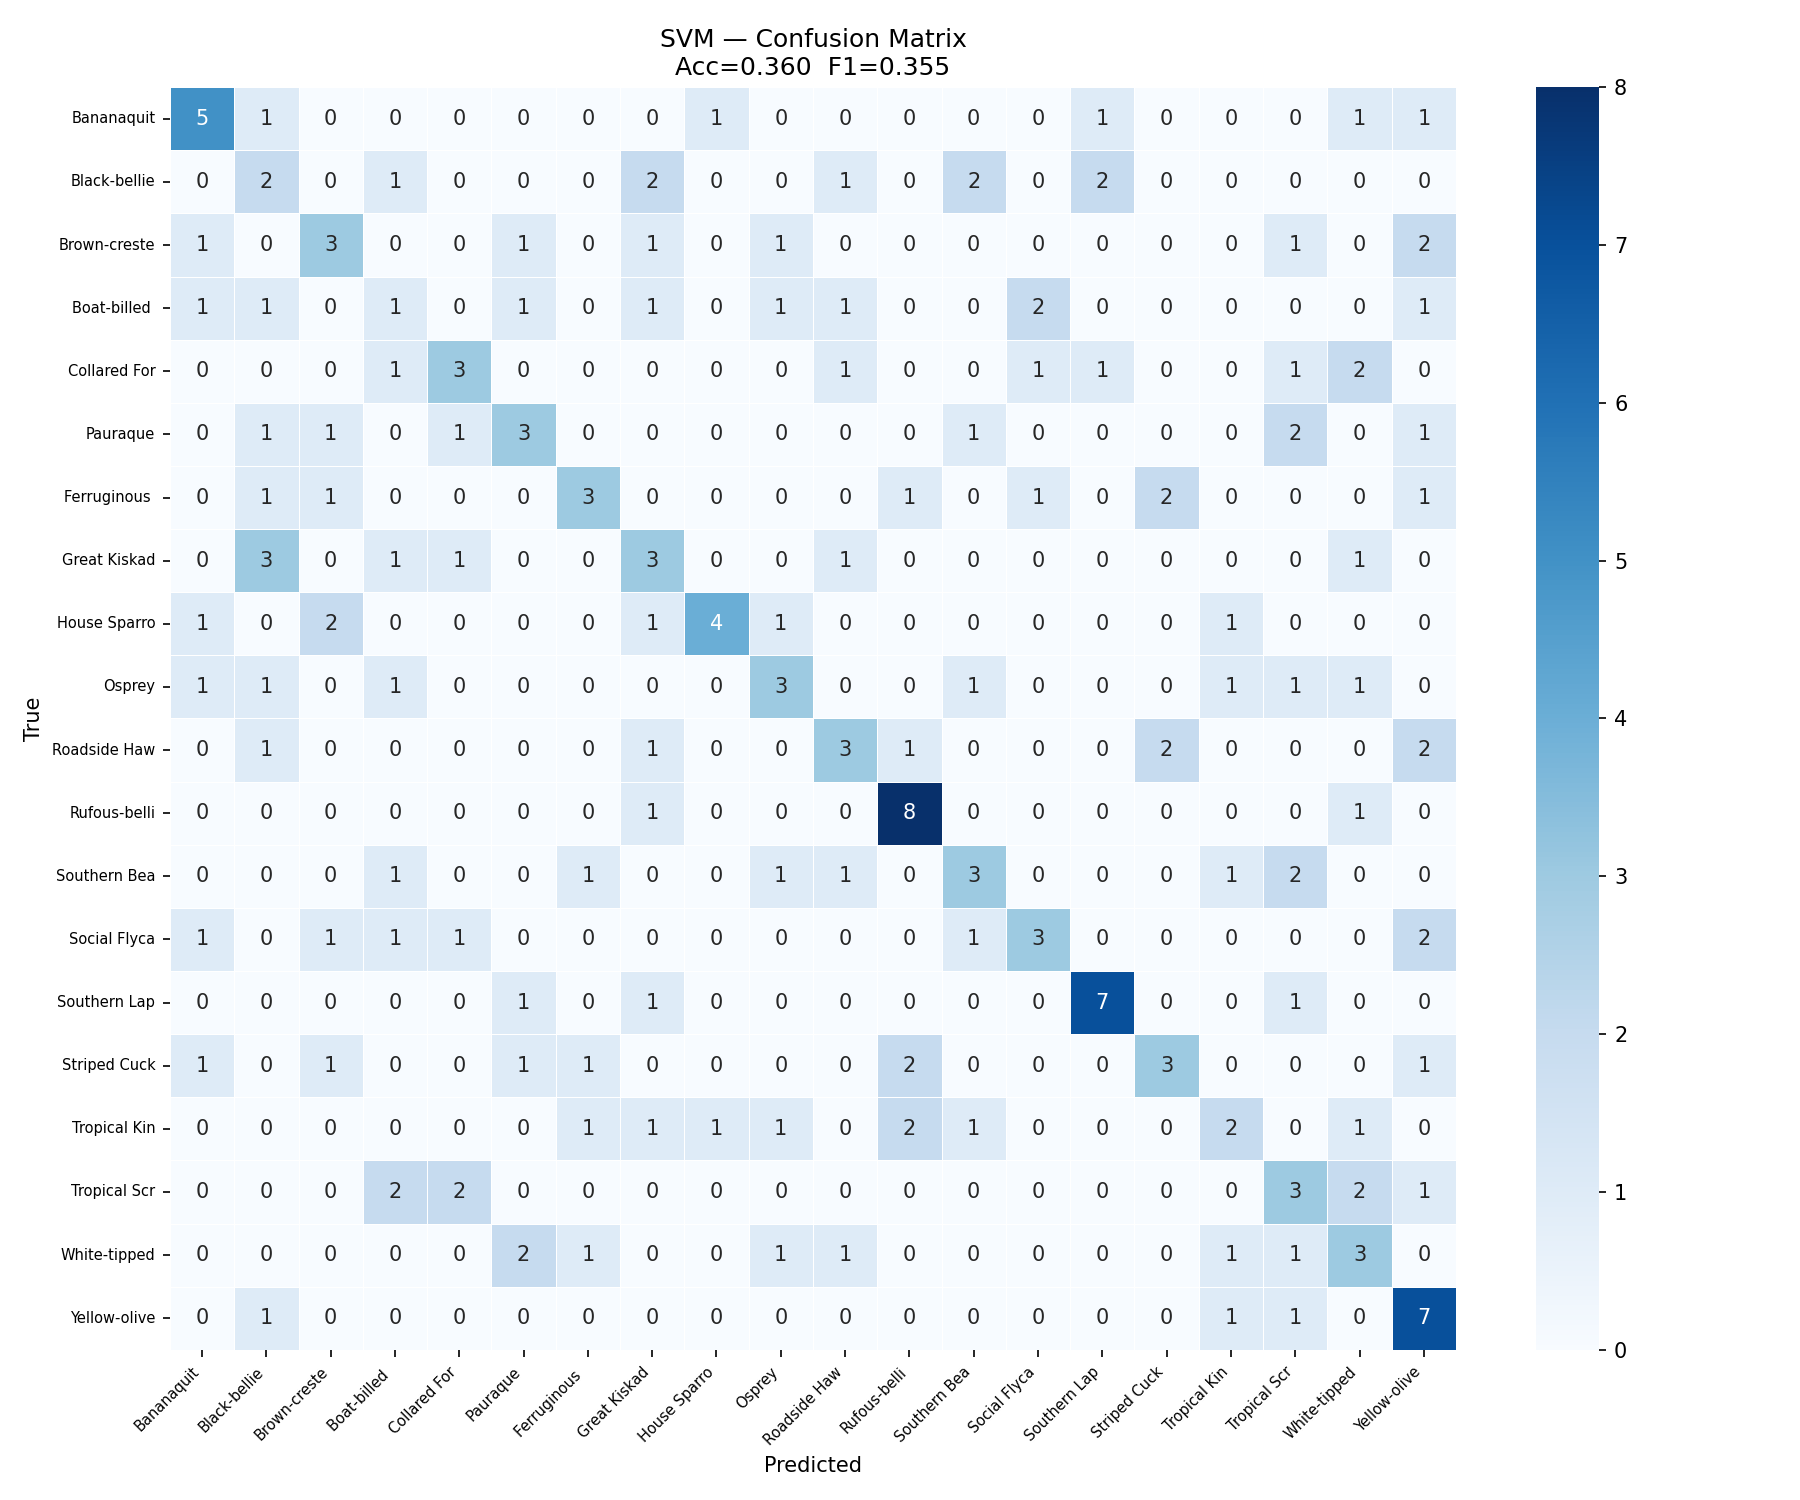
\includegraphics[width=\linewidth]{cm_svm.png}
\caption{SVM混淆矩阵（测试集，20类）}
\label{fig:cm_svm}
\end{figure}

\subsection{深度学习结果}

表~\ref{tab:dl_results}为两种深度学习模型的性能。
CNN以48.75\%的测试准确率成为所有模型中最优者，
BiLSTM以38.75\%紧随其后。

\begin{table}[h]
\caption{深度学习模型性能对比}
\label{tab:dl_results}
\centering\zihao{-5}
\resizebox{\columnwidth}{!}{%
\begin{tabular}{llll}
\toprule
模型 & 测试准确率 & Macro F1 & 输入 \\
\midrule
CNN    & 48.75\% & 0.463 & 梅尔频谱图$(1\!\times\!128\!\times\!212)$ \\
BiLSTM & 38.75\% & 0.385 & MFCC序列$(212\!\times\!40)$ \\
\bottomrule
\end{tabular}%
}
\end{table}

图~\ref{fig:cnn_curve}展示了CNN的训练曲线，
验证集准确率在约第15个epoch后趋于稳定，早停机制有效防止了过拟合。

\begin{figure}[h]
\centering
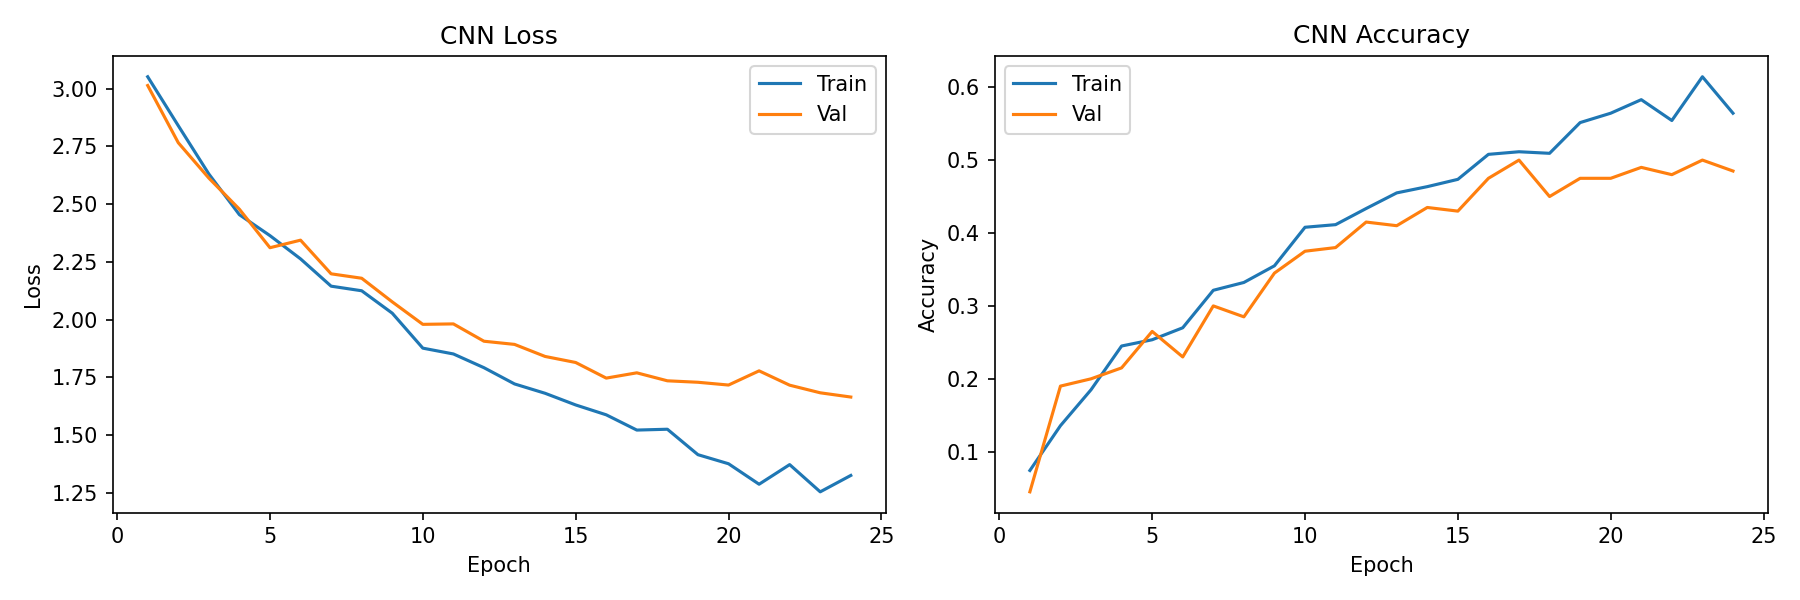
\includegraphics[width=\linewidth]{cnn_training_curves.png}
\caption{CNN训练曲线（损失与准确率随训练轮次的变化）}
\label{fig:cnn_curve}
\end{figure}

\begin{figure}[h]
\centering
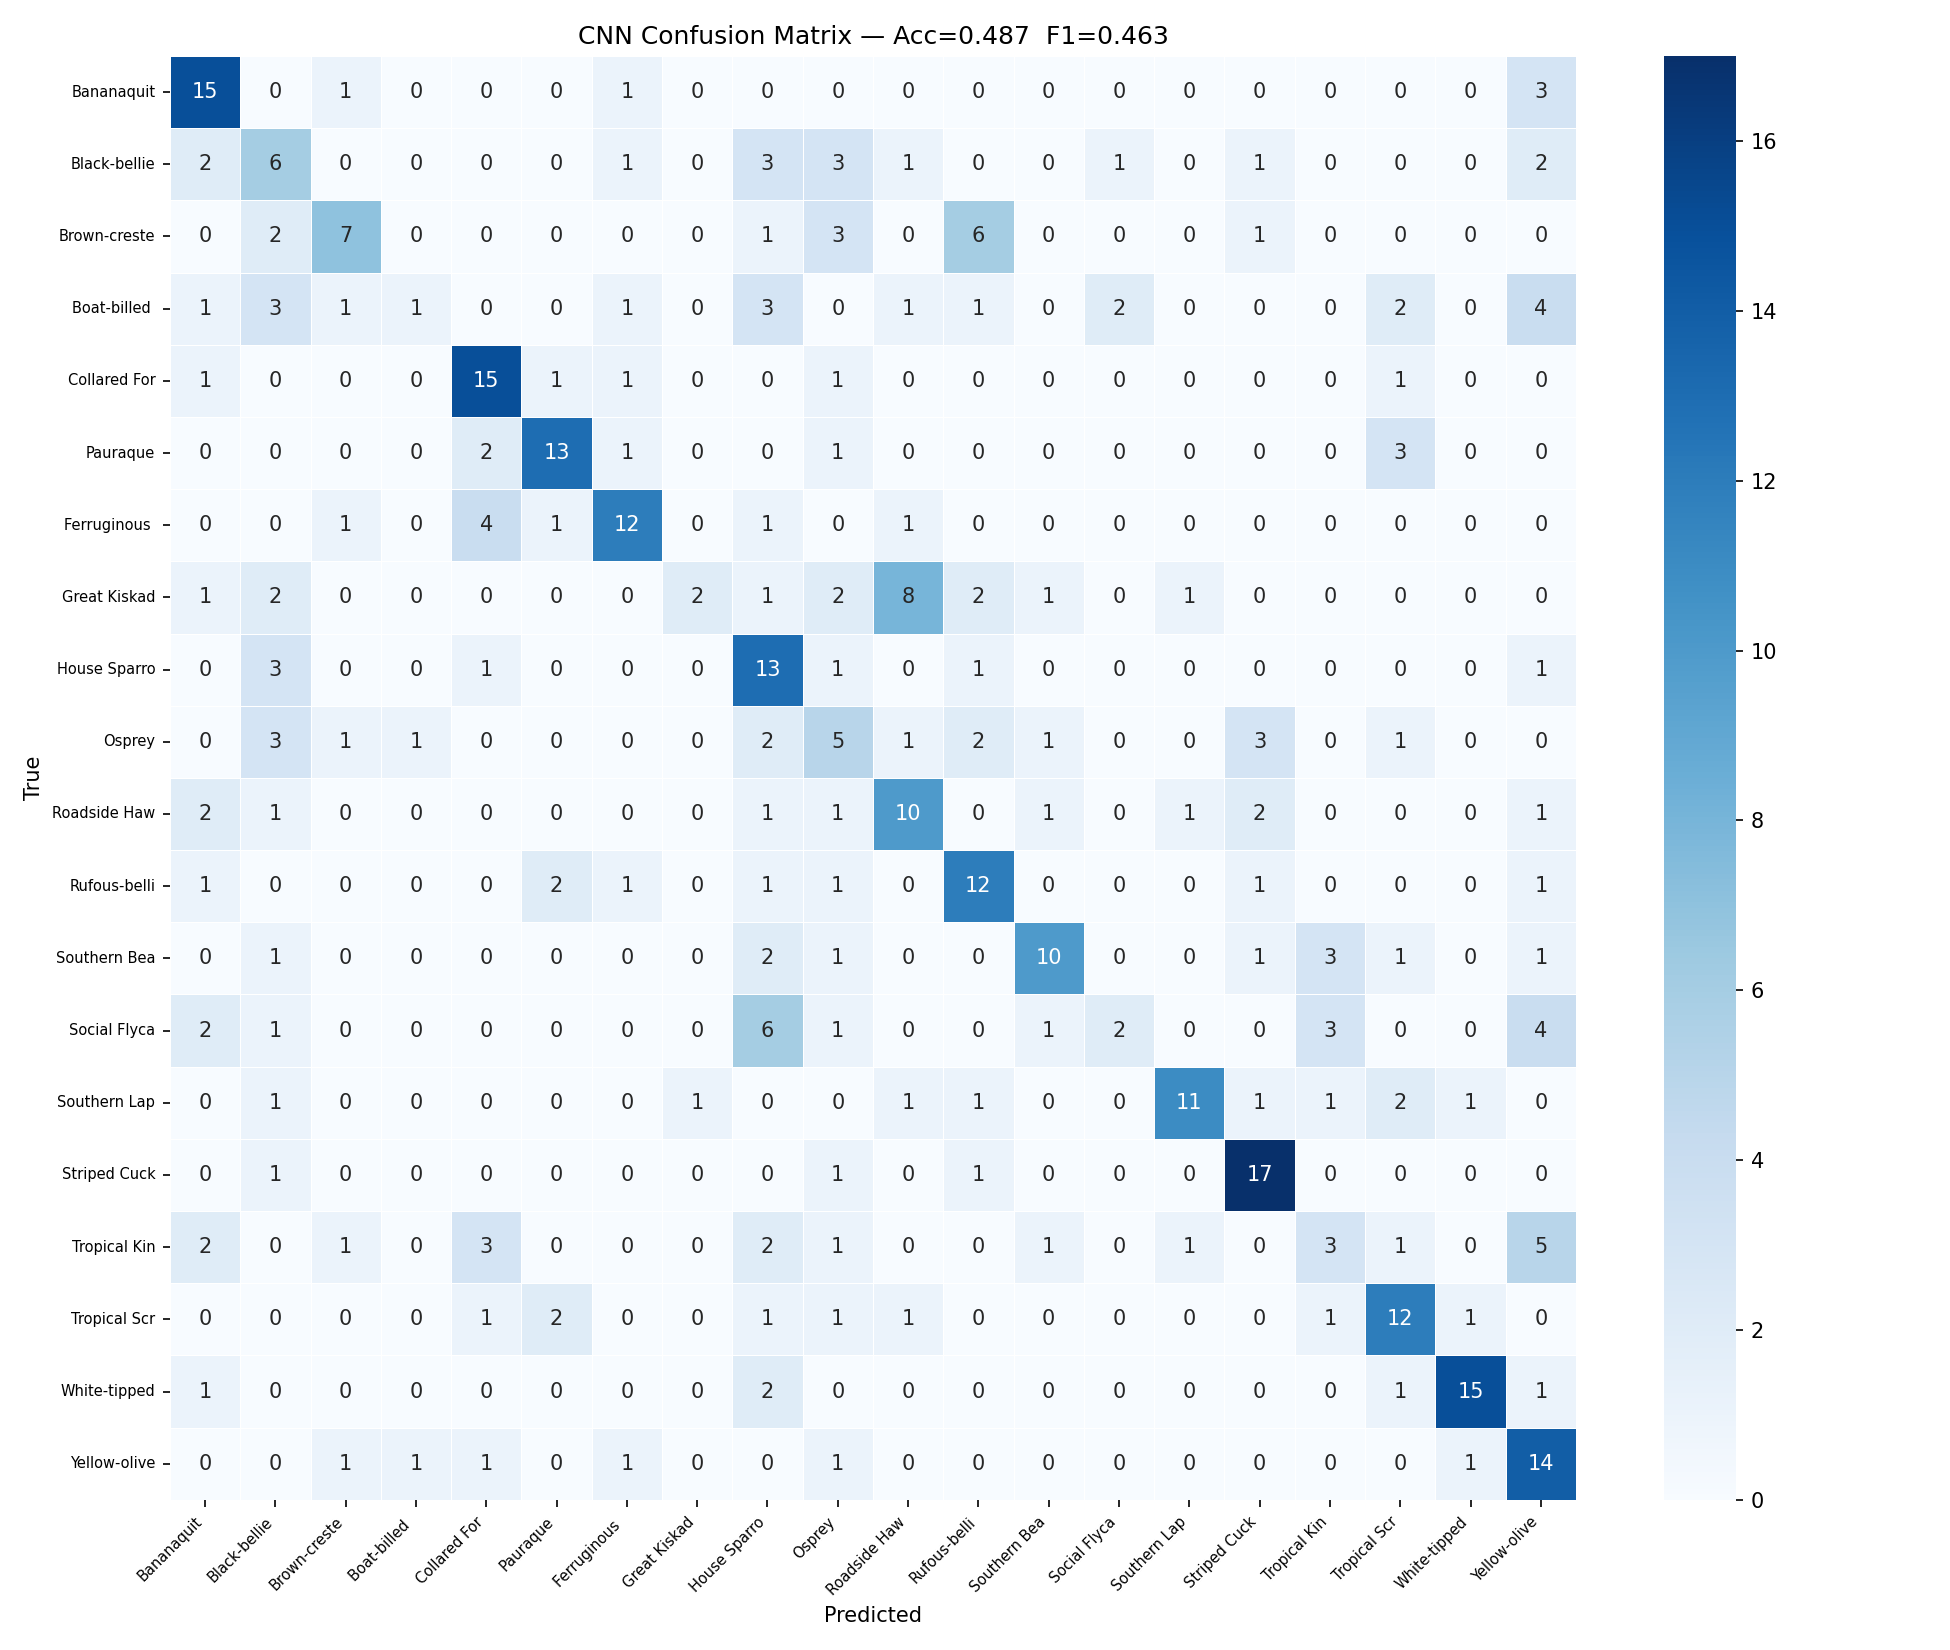
\includegraphics[width=\linewidth]{cnn_confusion_matrix.png}
\caption{CNN混淆矩阵（测试集，20类）}
\label{fig:cm_cnn}
\end{figure}

\subsection{综合对比与分析}

表~\ref{tab:all_results}给出了5种模型的综合排名，
图~\ref{fig:comparison}为对比柱状图。

\begin{table}[h]
\caption{五种模型综合性能排名}
\label{tab:all_results}
\centering\zihao{-5}
\begin{tabular}{lllll}
\toprule
排名 & 模型 & 类型 & 测试准确率 & Macro F1 \\
\midrule
1 & CNN    & 深度学习 & 48.75\% & 0.463 \\
2 & BiLSTM & 深度学习 & 38.75\% & 0.385 \\
3 & SVM    & 传统ML   & 36.00\% & 0.355 \\
4 & RF     & 传统ML   & 32.50\% & 0.314 \\
5 & KNN    & 传统ML   & 22.00\% & 0.209 \\
\bottomrule
\end{tabular}
\end{table}

\begin{figure}[h]
\centering
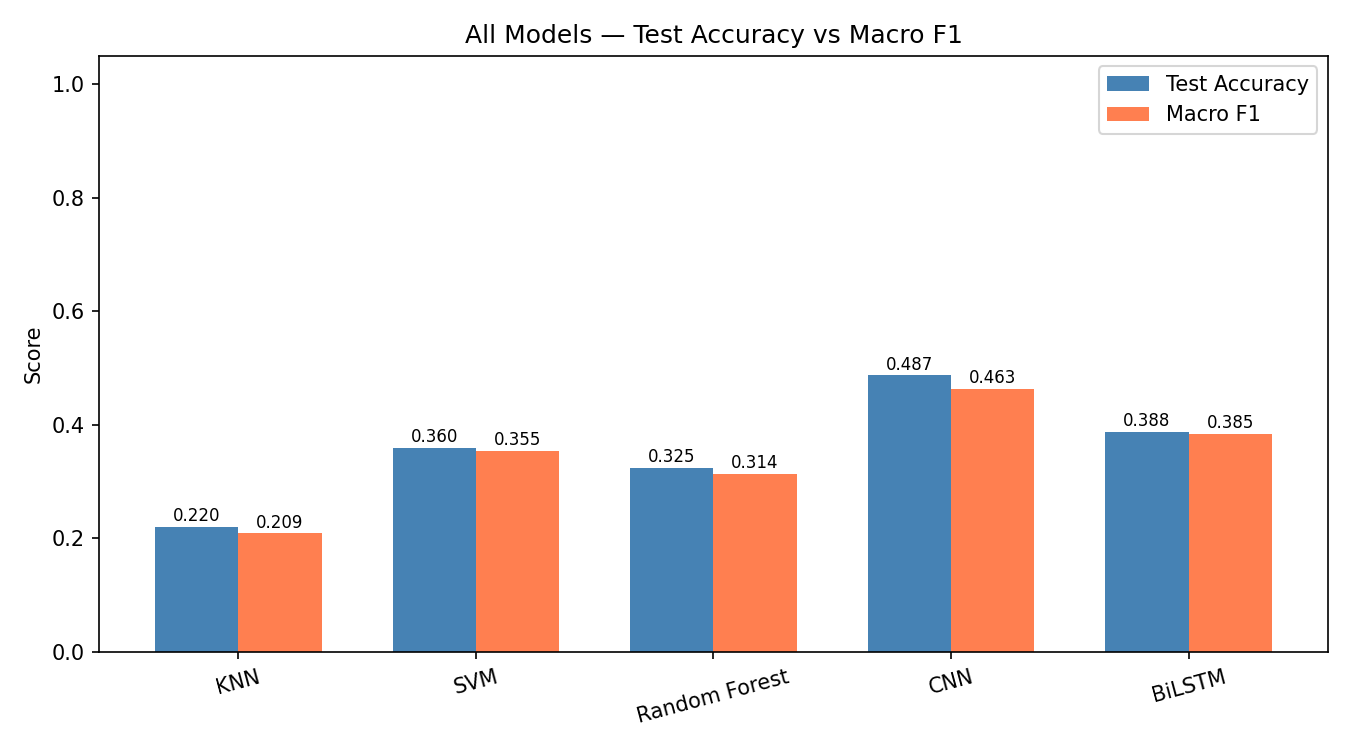
\includegraphics[width=\linewidth]{final_comparison.png}
\caption{五种模型测试集准确率与Macro F1综合对比}
\label{fig:comparison}
\end{figure}

深度学习整体优于传统机器学习，原因在于CNN和BiLSTM
能够直接从原始时频表示中自动学习判别特征，
而传统机器学习依赖手工统计特征，丢失了大量时序结构信息。
CNN优于BiLSTM，是因为对数梅尔频谱图保留了完整的二维时频结构，
卷积核可高效捕获局部时频模式。

整体准确率偏低的主要原因：
（1）每类训练样本仅50--100条，深度模型难以充分拟合；
（2）部分物种鸣声频率相似，区分难度较高（由混淆矩阵可见
Osprey与Tropical Screech Owl之间存在明显混淆）；
（3）实验在CPU上进行，模型规模和训练轮数受限。

% ════════════════════════════════════════════════════════════
\section{用户界面}

该文使用Gradio 4.x构建了基于Web的交互式识别界面，
支持上传.ogg/.wav/.mp3格式鸟鸣录音，
一键运行全部5个模型并同时展示结果。
界面主要包含：
（1）音频上传与播放区；
（2）音频可视化面板（波形/对数梅尔频谱/MFCC三合一图）；
（3）声学特征摘要（时长/平均音高/音量/过零率）；
（4）各模型Top-5物种识别结果与置信度百分比。
运行命令为\texttt{python 06\_ui.py}，访问\texttt{http://localhost:7860}。

% ════════════════════════════════════════════════════════════
\section{结论}

该文基于BirdCLEF 2026数据集实现了完整的鸟类鸣声识别系统，
涵盖数据预处理、278维多维声学特征提取、
5种模型（KNN/SVM/RF/CNN/BiLSTM）的构建与对比，
以及Web交互界面。
实验表明CNN（48.75\%）取得最优性能，
深度学习整体优于传统机器学习。
未来可通过以下方式进一步提升识别准确率：
（1）对训练音频施加时间拉伸、音调偏移、噪声叠加等数据增强；
（2）引入预训练音频模型（如BirdNET\cite{kahl2021}）进行迁移学习；
（3）对CNN、BiLSTM、SVM三模型的预测概率进行加权融合；
（4）引入Transformer等更强序列建模结构。

% ════════════════════════════════════════════════════════════
\begin{thebibliography}{99}
\zihao{-5}

\bibitem{stowell2019}
Stowell D, Wood M D, Pamuła H, et al.
Automatic acoustic detection of birds through deep learning:
the first Bird Audio Detection challenge[J].
Methods in Ecology and Evolution, 2019, 10(3): 368--380.

\bibitem{birdclef2026}
BirdCLEF 2026 Competition[EB/OL].
[2026-06-01].
https://www.kaggle.com/competitions/birdclef-2026.

\bibitem{mfcc1980}
Davis S, Mermelstein P.
Comparison of parametric representations for monosyllabic word recognition
in continuously spoken sentences[J].
IEEE Transactions on Acoustics, Speech, and Signal Processing,
1980, 28(4): 357--366.

\bibitem{yin2002}
De Cheveigné A, Kawahara H.
YIN, a fundamental frequency estimator for speech and music[J].
The Journal of the Acoustical Society of America,
2002, 111(4): 1917--1930.

\bibitem{cover1967}
Cover T, Hart P.
Nearest neighbor pattern classification[J].
IEEE Transactions on Information Theory, 1967, 13(1): 21--27.

\bibitem{cortes1995}
Cortes C, Vapnik V.
Support-vector networks[J].
Machine Learning, 1995, 20(3): 273--297.

\bibitem{breiman2001}
Breiman L. Random forests[J].
Machine Learning, 2001, 45(1): 5--32.

\bibitem{hochreiter1997}
Hochreiter S, Schmidhuber J.
Long short-term memory[J].
Neural Computation, 1997, 9(8): 1735--1780.

\bibitem{he2016}
He K, Zhang X, Ren S, et al.
Deep residual learning for image recognition[C]//
Proceedings of the IEEE Conference on Computer Vision
and Pattern Recognition. Las Vegas: IEEE, 2016: 770--778.

\bibitem{kahl2021}
Kahl S, Wood C M, Eibl M, et al.
BirdNET: A deep learning solution for avian diversity monitoring[J].
Ecological Informatics, 2021, 61: 101236.

\bibitem{mcfee2015}
McFee B, Raffel C, Liang D, et al.
librosa: Audio and music signal analysis in python[C]//
Proceedings of the 14th Python in Science Conference.
Austin: SciPy, 2015: 18--25.

\end{thebibliography}


\end{document}
